\documentclass[varwidth=true, border=2pt]{standalone}

\usepackage{pgfplots}
\usepackage{tikz}

\begin{document}
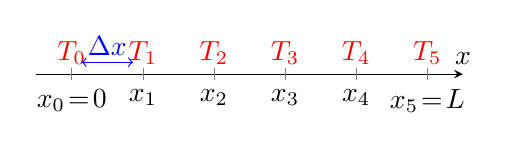
\begin{tikzpicture}
    \begin{axis}[
        legend pos=south east,
        axis x line=middle,
        axis y line=none,
	every axis x label/.style={at={(current axis.right of origin)},anchor=south},
	every axis y label/.style={at={(current axis.above origin)},anchor=east},
	every extra x tick/.style={xticklabel style={color=red,yshift=0.5ex, anchor=south}},
	yticklabels=\empty
        grid = none ,
        width=7cm,
        height=4cm,
        grid style={dashed, gray!1},
        xmin=0,     % start the diagram at this x-coordinate
        xmax=4,    % end   the diagram at this x-coordinate
        ymin=-1,     % start the diagram at this y-coordinate
        ymax=1,   % end   the diagram at this y-coordinate
        xlabel=$x$,
        ylabel=\empty,
        xtick={0,0.8,...,6},
        xticklabels={$x_0\! = \!0$,$x_1$,$x_2$,$x_3$,$x_4$,$x_5\! =\! L$},
        extra x ticks ={0,0.8,...,6},
        extra x tick labels={$T_0$,$T_1$,$T_2$,$T_3$,$T_4$,$T_5$},
        enlargelimits=true,
        tension=0.08]

	\node (x1) at  (axis cs: 0,0.15) {};
	\node (x2) at  (axis cs: 0.8,0.15) {};
	\node (x3)[blue] at  (axis cs: 0.4,0.35) {$\Delta x$};
	\draw [blue, <->] (x1)-- (x2);
   
    \end{axis}
\end{tikzpicture}
\end{document}